\documentclass[11pt,a4paper,oneside,openany,indonesian]{report}
\usepackage[a4paper,top=25mm,bottom=25mm,left=30mm,right=25mm,headheight=16pt,headsep=7mm,footskip=12mm]{geometry}
\usepackage{iftex}
\ifLuaTeX
  \usepackage[bidi=basic,shorthands=off,provide=*]{babel}
\else
  \usepackage[bidi=default,shorthands=off,provide=*]{babel}
\fi
\ifPDFTeX\else\babelfont{rm}[]{Charter}\fi
\usepackage{hyperref}
% Shared preamble for the Jakarta TGA chapters.
\usepackage{xcolor}
\usepackage{graphicx}
\usepackage{amsmath,amssymb}
\usepackage{iftex}
\ifPDFTeX
  \usepackage[T1]{fontenc}
  \usepackage[utf8]{inputenc}
  \usepackage{textcomp}
\else
  \usepackage{unicode-math}
  \defaultfontfeatures{Scale=MatchLowercase}
  \defaultfontfeatures[\rmfamily]{Ligatures=TeX,Scale=1}
\fi
\usepackage{lmodern}
\ifPDFTeX\else
  \setmainfont[]{Times New Roman}
  \setsansfont[]{Arial}
  \IfFontExistsTF{Consolas}{\setmonofont[]{Consolas}}{\setmonofont[]{Courier New}}
\fi
\IfFileExists{microtype.sty}{\usepackage{microtype}}{}
\usepackage{longtable,booktabs,array,tabularx,adjustbox,calc}
\usepackage{pdflscape}
\usepackage{caption}
\captionsetup[table]{skip=6pt}
\newcounter{none}
\usepackage{float}
\usepackage{setspace}
\usepackage{ragged2e}
\usepackage{titlesec}
\usepackage{enumitem}
\usepackage{needspace}
\usepackage{fancyhdr}
\usepackage{newunicodechar}
\usepackage{bookmark}
\usepackage{xurl}
\usepackage{csquotes}
\usepackage[backend=biber,style=authoryear,maxcitenames=2,maxbibnames=99,uniquelist=false,uniquename=false]{biblatex}
\DeclareLanguageMapping{indonesian}{english}
\DefineBibliographyStrings{english}{and={dan},andothers={dkk\adddot}}
\DefineBibliographyStrings{indonesian}{and={dan},andothers={dkk\adddot}}
\AtBeginDocument{\renewcommand*{\finalnamedelim}{\addspace dan\space}}
\addbibresource{references.bib}
\DeclareFieldFormat{title}{#1}
\DeclareFieldFormat[article,inbook,incollection,inproceedings,inreference,patent,thesis,unpublished]{title}{#1}
\AtBeginBibliography{\small\setlength{\bibitemsep}{0.15em}}

\newunicodechar{∅}{\ensuremath{\varnothing}}

% Placeholder untuk gambar yang dibuat manual (peta GIS). Ganti dengan \includegraphics setelah berkas target tersedia.
\newcommand{\GambarPlaceholder}[2][7cm]{%
  \fbox{\parbox[c][#1][c]{0.92\linewidth}{\centering\small
    \textbf{PLACEHOLDER GAMBAR}\\[0.6em]#2}}}

\definecolor{Ink}{HTML}{222222}
\definecolor{RuleGray}{HTML}{666666}

\AtBeginDocument{%
  \hypersetup{linkcolor=Ink,citecolor=Ink,urlcolor=Ink,pdfborder={0 0 0}}%
  \urlstyle{same}%
}

\setstretch{1.5}
\setlength{\parindent}{1.1em}
\setlength{\parskip}{0.28em}
\setlength{\emergencystretch}{2.5em}
\clubpenalty=10000
\widowpenalty=10000
\displaywidowpenalty=10000
\raggedbottom

\setlist[itemize]{leftmargin=1.7em,itemsep=0.25em,topsep=0.35em}
\setlist[enumerate]{leftmargin=1.9em,itemsep=0.25em,topsep=0.35em}

\titleformat{\chapter}[display]
  {\normalfont\bfseries\centering\color{Ink}}
  {}{0pt}{\Large\hyphenpenalty=10000\exhyphenpenalty=10000}
\titlespacing*{\chapter}{0pt}{-6pt}{18pt}
\titleformat{\section}{\Needspace{4\baselineskip}\large\bfseries\color{Ink}}{\thesection}{0.7em}{}
\titleformat{\subsection}{\Needspace{3\baselineskip}\normalsize\bfseries\color{Ink}}{\thesubsection}{0.7em}{}
\titleformat{\subsubsection}{\Needspace{3\baselineskip}\normalsize\bfseries\color{Ink}}{\thesubsubsection}{0.7em}{}

\pagestyle{plain}
\fancyhf{}
\fancyfoot[C]{\thepage}
\renewcommand{\headrulewidth}{0pt}
\renewcommand{\footrulewidth}{0pt}
\fancypagestyle{plain}{%
  \fancyhf{}
  \fancyfoot[C]{\thepage}
  \renewcommand{\headrulewidth}{0pt}
}

\renewcommand{\arraystretch}{1.2}
\setlength{\extrarowheight}{1pt}
\setlength{\tabcolsep}{4pt}
\providecommand{\tightlist}{\setlength{\itemsep}{0pt}\setlength{\parskip}{0pt}}
\setlength{\LTpre}{0.5em}
\setlength{\LTpost}{0.8em}
\AtBeginEnvironment{longtable}{\footnotesize\setstretch{1.0}\setlength{\tabcolsep}{3pt}\setlength{\extrarowheight}{1pt}}
\AtBeginEnvironment{table}{\setstretch{1.0}}
\AtBeginEnvironment{figure}{\setstretch{1.0}}
\AtBeginEnvironment{quote}{\small\setlength{\leftskip}{1.2em}\setlength{\rightskip}{1.2em}}


\hypersetup{
  pdftitle={Bab 3 Metode Penelitian},
  pdfauthor={Mahastri Laksita Sam Widita},
  pdflang={id-ID},
  hidelinks
}

\title{\textbf{Borrowed Size atau Agglomeration Shadow?}\\[0.4em]
Analisis Hubungan Integrasi Metropolitan dengan Kematangan Pusat-Pusat Sekunder di Kawasan Aglomerasi Jakarta}
\providecommand{\subtitle}[1]{\gdef\thesubtitle{#1}}
\subtitle{Bab 3 Metode Penelitian}
\author{Mahastri Laksita Sam Widita\\NIM 22/503065/TK/54947\\[0.5em]
Pembimbing: Rendy Bayu Aditya\\[0.5em]
Program Studi Perencanaan Wilayah dan Kota\\
Departemen Teknik Arsitektur dan Perencanaan\\
Fakultas Teknik\\
Universitas Gadjah Mada}
\date{Kabupaten Sleman, Daerah Istimewa Yogyakarta\\2026}

\makeatletter
\renewcommand{\maketitle}{%
  \begin{titlepage}
    \centering
    {\Large\bfseries TUGAS AKHIR\par}
    \vfill
    {\LARGE\bfseries \@title\par}
    \vspace{1.2cm}
    {\large \thesubtitle\par}
    \vfill
    {\large \@author\par}
    \vfill
    {\large \@date\par}
  \end{titlepage}}
\makeatother

\begin{document}
\maketitle
\tableofcontents
\clearpage
\setcounter{chapter}{2}
\chapter{Metode Penelitian}
\section{Pendekatan penelitian}\label{pendekatan-penelitian}

\subsection{Pilihan pendekatan}\label{pilihan-pendekatan}

Penelitian ini menggunakan pendekatan kuantitatif deduktif dengan
analisis spasial-relasional. Konstruk integrasi metropolitan,
fungsi relatif, manfaat, beban, serta gerbang penggunaan label
\emph{borrowed size} dan \emph{agglomeration shadow} diturunkan dari
kerangka konseptual Bab 2 sebelum klasifikasi dilakukan. Pendekatan ini
dipilih karena pertanyaan penelitian menuntut pengukuran hubungan antara
pusat sekunder dan Jakarta, perbandingan fungsi aktual dengan fungsi
yang diharapkan dari ukuran lokal, serta pengujian stabilitas hasil pada
variasi asumsi.

Pendekatan ini tidak berarti semua konstruk harus direduksi menjadi satu
angka. Integrasi, fungsi relatif, manfaat, ketergantungan, dan beban
dipertahankan sebagai dimensi yang dapat dibaca bersama. Statistik
deskriptif, pemetaan, analisis jaringan, tolok ukur, residu, dan uji
sensitivitas digunakan sesuai jenis bukti yang tersedia.

Audit dokumen dan audit asal-usul data merupakan prosedur penjaminan
mutu. Prosedur ini digunakan untuk memeriksa definisi, tahun, unit,
cakupan, cara pembentukan, nilai hilang, dan batas penggunaan data.
Pemeriksaan dokumen tersebut tidak menjadikan penelitian ini penelitian
campuran karena dokumen tidak dianalisis sebagai data untuk menjawab
pertanyaan substantif. Angka dalam laporan publik dapat diekstrak sebagai
data sekunder apabila tabel atau pernyataan sumber, unit, dan periodenya
dapat ditelusuri. Kekosongan angka tidak diisi dengan dugaan yang
disamarkan sebagai pengamatan.

\subsection{Alasan kesesuaian dengan pertanyaan
penelitian}\label{alasan-kesesuaian-dengan-pertanyaan-penelitian}

Kesesuaian pendekatan dengan pertanyaan penelitian diringkas sebagai
berikut.

{\def\LTcaptype{none} % do not increment counter
\begin{longtable}[]{@{}
  >{\raggedright\arraybackslash}p{(\linewidth - 4\tabcolsep) * \real{0.3333}}
  >{\raggedright\arraybackslash}p{(\linewidth - 4\tabcolsep) * \real{0.3333}}
  >{\raggedright\arraybackslash}p{(\linewidth - 4\tabcolsep) * \real{0.3333}}@{}}
\toprule\noalign{}
\begin{minipage}[b]{\linewidth}\raggedright
Kode
\end{minipage} & \begin{minipage}[b]{\linewidth}\raggedright
Fokus pertanyaan
\end{minipage} & \begin{minipage}[b]{\linewidth}\raggedright
Alasan menggunakan pendekatan kuantitatif-spasial
\end{minipage} \\
\midrule\noalign{}
\endhead
\bottomrule\noalign{}
\endlastfoot
Q1 & Arah, intensitas, dan asimetri hubungan metropolitan & Pengamatan
dan estimasi relasi dari sumber terbuka dibandingkan pada unit yang
sah. \\
Q2 & Fungsi relatif, manfaat, beban, dan perubahan pada seri sebanding &
Pengukuran atau estimasi fungsi dibandingkan dengan tolok ukur, sementara
manfaat dan beban dilaporkan pada penerima serta penanggungnya. \\
Q3 & Hubungan integrasi dan fungsi relatif serta konfigurasi hasil &
Asosiasi, heterogenitas antarpusat, sirkularitas, kondisi lokal, dan
penjelasan alternatif diperiksa sebelum diagnosis. \\
\end{longtable}
}

Sensitivitas menjadi pemeriksaan lintas ketiga pertanyaan, bukan
pertanyaan substantif tersendiri.

Pendekatan ini tidak cukup untuk menyatakan dampak kausal pembangunan
jalan, perluasan wilayah, atau kebijakan tertentu tanpa strategi
identifikasi tambahan. Karena itu, istilah yang dipakai dalam Bab 3
adalah \emph{asosiasi}, \emph{pola}, \emph{surplus atau defisit
relatif}, \emph{ketergantungan yang konsisten dengan data}, dan
\emph{ketahanan klasifikasi}, bukan ``dampak kausal'' kecuali desain
kelak benar-benar diperkuat.

\subsection{Fondasi pengukuran}\label{fondasi-pengukuran}

Penelitian ini sepenuhnya bertumpu pada proksi dan sumber terbuka, tanpa
ketergantungan pada permohonan data tertutup. Data pemerintah yang
terbuka tetap dapat digunakan. Pemilihan sumber mengikuti kesesuaian
konstruk, cakupan spasial dan temporal, keterulangan pengolahan, serta
biaya pemerolehan; status resmi tidak menjadi ukuran mutu dengan
sendirinya. Sumber alternatif dapat lebih sesuai daripada data resmi
agregat yang tersedia, tetapi keunggulan tersebut diuji per konstruk dan
tidak diasumsikan berlaku universal.

\section{Desain penelitian}\label{desain-penelitian}

\subsection{Bentuk desain}\label{bentuk-desain}

Penelitian dirancang sebagai studi kasus tunggal kuantitatif-spasial
dengan pengamatan multitemporal sesuai bukti, diagnosis relasional, dan
analisis sensitivitas. Kasus tunggal dipilih agar pusat-pusat sekunder
dapat dibandingkan di dalam satu sistem metropolitan tanpa memperlakukan
perbedaan antarmetropolitan sebagai variasi yang setara. Populasi
pembanding utama adalah pusat-pusat sekunder di dalam Jabodetabek yang
memiliki konstruk, unit, dan periode sebanding. DKI Jakarta dikeluarkan
dari pembentukan ekspektasi karena kedudukannya sebagai inti. Sabuk
pembanding di luar kawasan studi hanya digunakan sebagai pemeriksaan
sensitivitas apabila definisi, unit, dan periodenya kompatibel.

Desain ini bekerja melalui tiga lapisan:

\begin{enumerate}
\def\labelenumi{\arabic{enumi}.}
\tightlist
\item
  Lapisan pengukuran membedakan observasi langsung atau agregat, proksi,
  serta hasil estimasi yang dibedakan secara eksplisit pada unit dan
  periode yang tercantum dalam manifest.
\item
  Lapisan diagnosis mengukur integrasi, fungsi relatif,
  manfaat, beban, dan tipologi dari satu konfigurasi bukti yang
  dibekukan.
\item
  Lapisan ketahanan dan eksplorasi menguji perubahan konfigurasi
  bukti, spesifikasi model, atau nilai skenario yang dibatasi dan selalu
  dilaporkan terhadap garis dasar tanpa menimpa data observasi.
\end{enumerate}

\subsection{Urutan kerja
penelitian}\label{urutan-kerja-penelitian}

Penelitian dilaksanakan melalui delapan tahap yang saling terkait.

\begin{enumerate}
\def\labelenumi{\arabic{enumi}.}
\tightlist
\item
  Menginventarisasi sumber dan mencatat asal-usul setiap data.
\item
  Mengaudit konstruk, tahun, unit, cakupan, lisensi, nilai hilang, dan
  batas penggunaan.
\item
  Mengharmonisasi geometri dan tabel, kemudian membekukan konfigurasi
  bukti garis dasar.
\item
  Membentuk kandidat pusat, wilayah tangkapan, relasi terarah, dan
  residu fungsi per domain.
\item
  Menganalisis asosiasi, manfaat, beban, dan ketergantungan tanpa
  meleburkan dimensi yang berbeda.
\item
  Menerapkan gerbang bukti sebelum memberi label diagnosis.
\item
  Menguji sensitivitas indikator, bobot, ambang, unit, dan konfigurasi
  bukti.
\item
  Menyusun tabel, peta, manifest, dan batas klaim yang dapat diperiksa
  ulang; Web GIS interaktif hanya disiapkan jika keluaran inti telah
  selesai dan waktu penelitian memungkinkan.
\end{enumerate}

\begin{figure}[H]
  \centering
  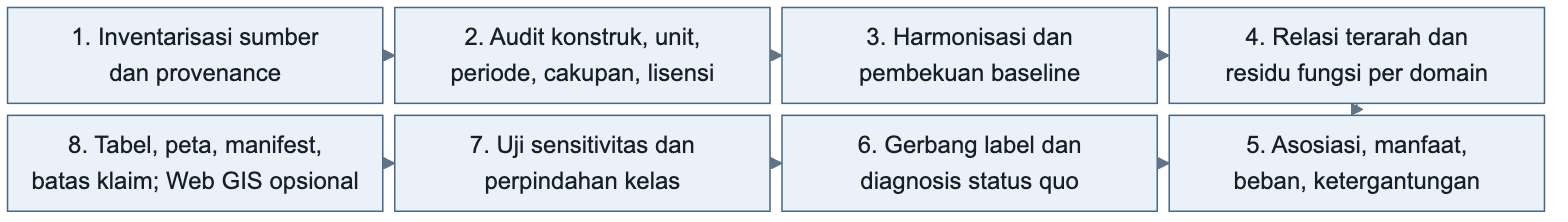
\includegraphics[width=\textwidth]{figures/bab3_alur_analisis.png}
  \caption{Alur analisis dari inventarisasi sumber hingga penyusunan keluaran dan batas klaim. Setiap tahap dapat menurunkan tingkat klaim jika mutu atau keterbandingan bukti tidak memadai.}
  \label{fig:bab3-alur-analisis}
\end{figure}

\subsection{Rancangan analisis minimum}\label{rancangan-analisis-minimum}

Rancangan minimum dibatasi pada satu periode yang kompatibel, satu bukti
relasi komuter terarah, satu domain fungsi yang dibentuk secara
independen, tolok ukur internal Jabodetabek, serta pembacaan hubungan
antara relasi dan residu fungsi. Domain pekerjaan menjadi pilihan utama
jika pasangan arus komuter diamati tanpa dibentuk dari estimasi pekerjaan
yang sama. Layanan berorde tinggi dapat menjadi domain kedua apabila
atributnya lolos audit dan tidak digunakan untuk membentuk relasi.

Jika jumlah pusat efektif tidak memadai untuk regresi, keluaran minimum
berupa profil terarah dan perbandingan kelompok. Analisis multitemporal,
domain kedua, CCTV, SUMO, dan Web GIS interaktif dilaksanakan setelah
rantai utama tersebut berjalan dan tidak menjadi syarat untuk menjawab
pertanyaan inti. Kategori diagnosis hanya dibentuk jika keempat gerbang
bukti terpenuhi; hasil lain tetap sah sebagai profil relasi serta surplus
atau defisit fungsi relatif.

\subsection{Kelebihan dan keterbatasan
desain}\label{kelebihan-dan-keterbatasan-desain}

Desain memungkinkan pengukuran spasial terperinci dan pengamatan
beberapa periode dari sumber yang dapat diperiksa tanpa menunggu akses
kelembagaan. Keterbatasan data administratif maupun nonpemerintah
dinilai secara simetris. Ketersediaan koordinat, panjang seri, dan
banyaknya sumber merupakan keunggulan hanya sejauh membantu mengukur
konstruk yang dituju.

Galat klasifikasi usaha, duplikasi, cakupan yang berbeda antardaerah,
perubahan pencatatan, dan asumsi model dapat memengaruhi hasil.
Pemeriksaan independen, harmonisasi, serta propagasi ketidakpastian
digunakan untuk mengukur pengaruhnya. Data multitemporal tidak dengan
sendirinya mengidentifikasi sebab-akibat.

\subsection{Perbedaan diagnosis dan
skenario}\label{perbedaan-diagnosis-dan-skenario}

Nilai \emph{status quo} dibekukan sebagai garis dasar. Perubahan
penggeser atau parameter tidak boleh menimpa nilai observasi, mengubah
batas administratif, atau disajikan sebagai prediksi. Setiap skenario
menyimpan konfigurasi indikator, bobot, ambang, nilai yang diubah, dan
alasan substantif perubahan.

Perubahan karena sumber data diperoleh, hilang, atau turun mutu dicatat
sebagai skenario bukti. Perubahan bobot, ambang, atau
spesifikasi dalam konfigurasi bukti yang sama dicatat sebagai
skenario parameter. Perubahan nilai indikator untuk pertanyaan
\emph{what-if} merupakan eksplorasi kondisional tambahan. Ketiganya
tidak boleh ditampilkan sebagai jenis perubahan yang sama.

\section{Ruang lingkup penelitian}\label{ruang-lingkup-penelitian}

\subsection{Ruang lingkup spasial}\label{ruang-lingkup-spasial}

Kasus utama adalah Jabodetabek sebagai kawasan utama penelitian. Tolok
ukur utama dibentuk dari pusat sekunder yang sebanding di dalam kawasan
ini. Sabuk Wilayah Statistik Metropolitan di luar cakupan hanya menjadi
pemeriksaan sensitivitas apabila datanya kompatibel. Kasus ini dipilih karena memungkinkan
hubungan antara satu inti dan kandidat pusat sekunder lintas batas
administratif diperiksa di dalam sistem metropolitan yang sama. DKI
Jakarta diperlakukan sebagai satu inti untuk hubungan eksternal, dengan
batas administratif tetap. Data rinci di dalam DKI tetap dapat digunakan
untuk pemeriksaan internal, tetapi tidak mengubah keputusan bahwa DKI
diperlakukan sebagai satu inti dalam klasifikasi eksternal.

Wilayah di luar DKI tidak disebut sebagai ``wilayah Jakarta'' hanya
karena masuk dalam gradien analisis. Istilah yang digunakan adalah
jejak fungsional Jakarta, zona analitis keterkaitan metropolitan, atau
gradien integrasi-ketergantungan metropolitan. Istilah tersebut bukan zonasi legal RTRW dan tidak
mengubah kewenangan pemerintah daerah.

Seluruh wilayah administratif di sekitar Jakarta tidak diasumsikan
otomatis menjadi unit analisis yang tepat. Delineasi akhir harus
menjelaskan sumber, tahun, definisi, dan alasan memasukkan atau
mengeluarkan setiap unit.

\subsection{Ruang lingkup temporal}\label{ruang-lingkup-temporal}

Desain penelitian bersifat multitemporal sesuai bukti: perubahan
dianalisis pada indikator dengan seri yang sebanding, sedangkan
indikator lain dianalisis pada periode yang tersedia. Tahun dasar dan
rentang analisis ditetapkan per modul setelah audit; panel lengkap dan
satu tahun jangkar untuk semua sumber tidak diasumsikan.

Setiap modul menyimpan tahun observasi, tanggal ekstraksi, waktu
publikasi, dan periode berlakunya atribut. Analisis perubahan
mensyaratkan sedikitnya dua pengamatan yang sebanding; dua titik tidak
disebut tren tahunan. Riwayat suntingan OSM dan tanggal kemunculan dalam
direktori bukan otomatis tanggal berdiri atau tutup usaha. Data mutakhir
tidak diproyeksikan ke masa lalu tanpa model dan bukti. Seri tidak
sebanding dianalisis terpisah; interpolasi, jika digunakan, diberi label
estimasi dan tidak menambah jumlah observasi independen.

\subsection{Ruang lingkup
substantif}\label{ruang-lingkup-substantif}

Penelitian mencakup:

\begin{itemize}
\tightlist
\item
  Integrasi atau eksposur metropolitan;
\item
  Fungsi lokal dan fungsi relatif pada satu atau paling banyak dua
  domain inti;
\item
  Manfaat akses yang dapat diamati atau diproksikan secara sah;
\item
  Beban komuter dan ketergantungan yang diukur terpisah dari residu
  fungsi;
\item
  Tipologi \emph{borrowed size}, campuran,
  \emph{agglomeration shadow}, terintegrasi tetapi tertinggal, relatif
  independen, periferi lemah, dan tidak terselesaikan;
\item
  Sensitivitas indikator, bobot, ambang, unit, dan status mutu bukti;
  serta
\item
  Penyajian hasil dalam atlas, tabel, dan peta; Web GIS interaktif dapat
  ditambahkan sebagai media komunikasi.
\end{itemize}

Penelitian tidak mencakup penetapan radius geometris Jakarta,
rekomendasi perubahan batas administrasi, pembuktian kausal seluruh
kebijakan metropolitan, atau klaim produktivitas penuh jika fungsi
ekonomi pada unit yang sesuai tidak tersedia.

Kematangan dalam penelitian ini berarti kematangan fungsi lokal pada
domain yang benar-benar diukur. Konstruk tersebut tidak disamakan dengan
kesejahteraan penduduk, keterjangkauan layanan, mutu pelayanan secara
menyeluruh, ketahanan ekonomi, atau keberhasilan pembangunan. Akses,
manfaat, dan beban dilaporkan terpisah dan tidak digunakan untuk
memperluas arti residu fungsi.

\section{Unit amatan dan unit
analisis}\label{unit-amatan-dan-unit-analisis}

\subsection{Unit amatan}\label{unit-amatan}

Unit amatan adalah satuan tempat setiap observasi dicatat pada sumber.
Satuan tersebut dapat berupa desa/kelurahan, kecamatan, kabupaten/kota,
zona asal-tujuan, titik fasilitas, atau sel raster. Kecamatan menjadi
sasaran unit amatan utama untuk modul yang memiliki bukti relasional dan
fungsi yang kompatibel karena cukup rinci untuk membedakan kandidat
pusat sekunder dan wilayah sekitarnya.

Kecamatan tidak dipaksakan ketika data kritis hanya tersedia pada
kabupaten/kota atau zona model. Dalam keadaan tersebut, perhitungan
dilakukan pada unit sumber atau sebagai analisis paralel multiresolusi.
Alokasi nilai kabupaten/kota ke kecamatan, kisi, atau titik hanya
dilakukan dengan model eksplisit menggunakan informasi lokal, pemeriksaan
independen, dan ketidakpastian; hasil tetap merupakan estimasi, bukan
observasi rinci.

Kisi atau heksagon hanya digunakan untuk data yang berasal dari raster
atau titik, misalnya cahaya malam, morfologi terbangun, atau titik
minat. Kisi dapat menjadi unit perhitungan utama bagi modul yang
didukung titik atau raster. Resolusi keluaran mengikuti kemampuan
pengukuran; koordinat rinci tidak otomatis menjamin ketepatan nilai
atribut.

\subsection{Unit analisis
substantif}\label{unit-analisis-substantif}

Unit analisis substantif adalah kandidat pusat sekunder beserta wilayah
tangkapan fungsionalnya. Secara operasional, satu pusat dapat
direpresentasikan oleh satu kecamatan, beberapa unit yang bersebelahan,
atau zona sumber selama aturan pembentukannya dibekukan dan dapat
direproduksi. Kabupaten/kota tetap menjadi lapisan agregasi kebijakan,
layanan, APBD, dan tanggung jawab pemerintahan, tetapi tidak otomatis
menjadi pusat sekunder.

Daftar kandidat awal dibentuk dari konsentrasi aktivitas dan fungsi
dalam sumber terbuka, serta dibandingkan dengan pusat yang dikenali
dalam dokumen perencanaan. Penetapannya menggunakan bukti kepadatan
aktivitas, fungsi layanan, pekerjaan, kawasan industri, posisi jaringan,
atau arus yang tersedia. Variabel untuk delineasi dipisahkan dari
variabel hasil sejauh data memungkinkan. Jika indikator yang sama harus
digunakan pada kedua tahap, ketahanan klasifikasi diuji kembali dengan
mengeluarkan indikator tersebut agar penetapan pusat tidak menjadi
pembuktian sirkular.

\subsection{Aturan keterbandingan
unit}\label{aturan-keterbandingan-unit}

Setiap indikator dicatat dengan unit asli, unit perhitungan, unit
pelaporan, dan operasi transformasinya. Satu klasifikasi hanya dihitung
jika bukti relasional dan bukti fungsi dapat dipadankan pada unit,
wilayah tangkapan, dan periode yang sebanding atau dapat diagregasikan
secara sah. Harmonisasi mengikuti aturan:

\begin{enumerate}
\def\labelenumi{\arabic{enumi}.}
\tightlist
\item
  Gunakan unit asli untuk perhitungan awal;
\item
  Gunakan tabel korespondensi resmi jika tersedia;
\item
  Agregasikan unit rinci ke unit lebih kasar bila operasi tersebut sah;
\item
  Jalankan analisis paralel bila unit tidak dapat disetarakan;
\item
  Keluarkan modul jika keterbandingan tidak dapat dipertanggungjawabkan;
  dan
\item
  Jangan membandingkan skor lintas konfigurasi bukti sebagai perubahan
  kondisi tanpa menyatakan perbedaan sumber dan unitnya.
\end{enumerate}

\subsection{Populasi, cakupan, dan validasi
manual}\label{populasi-cakupan-dan-validasi-manual}

Populasi analisis adalah seluruh kandidat pusat dan wilayah tangkapan
yang masuk dalam delineasi akhir serta mempunyai bukti yang memenuhi
aturan modul. Jika sumber merupakan sensus atau inventaris seluruh unit,
penelitian tidak mengambil sampel statistik tambahan. Pemeriksaan manual
dilakukan secara purposif pada tiga sampai lima pusat sekunder prioritas
untuk memeriksa lokasi kampus dan rumah sakit; usaha dan titik minat
lain diperiksa pada sampel terarah yang mencakup variasi sektor,
koridor, dan tingkat ketercakupan. Audit silang memeriksa asal-usul
sumber agar dua salinan data yang sama tidak dianggap dua bukti
independen. Kriteria pemilihan pusat validasi dicatat sebelum
pemeriksaan. Validasi terbatas tersebut bukan sampel inferensial dan
tidak digeneralisasikan sebagai sensus seluruh kawasan.

Untuk tolok ukur fungsi, populasi pembanding garis dasar menggunakan
seluruh pusat sekunder yang lolos aturan keterbandingan pada domain yang
sama. Nilai suatu pusat diperkirakan dari pusat pembanding lain dengan
prosedur \emph{leave-one-out} agar pengamatan yang sedang dinilai tidak
menentukan ekspektasinya sendiri. Jika jumlah pusat tidak mendukung model
fungsi-ukuran, pembanding dibentuk dari kelompok ukuran atau tetangga
ukuran terdekat yang transparan. Kedua prosedur tetap menghasilkan
posisi relatif di dalam Jabodetabek.

\section{Metode pengumpulan data}\label{metode-pengumpulan-data}

\subsection{Prinsip pengumpulan
data}\label{prinsip-pengumpulan-data}

Penelitian ini sepenuhnya bertumpu pada proksi dan sumber terbuka, tanpa
ketergantungan pada permohonan data tertutup. Data pemerintah yang
terbuka tetap dapat digunakan. Pemilihan sumber mengikuti kesesuaian
konstruk, cakupan spasial dan temporal, keterulangan pengolahan, serta
biaya pemerolehan; status resmi tidak menjadi ukuran mutu dengan
sendirinya.

Akuisisi mengikuti sumber yang benar-benar dapat digunakan: unduhan,
layanan data, direktori publik, laporan operator, publikasi statistik,
serta ekstraksi dokumen dengan locator tabel atau halaman. Metode
pengambilan OSM dan Google Maps ditetapkan setelah audit kemampuan
akses; penelitian tidak menganggap satu endpoint pencarian sebagai
satu-satunya cara akuisisi atau hasil pencarian sebagai sensus lengkap.
Terlihat publik tidak otomatis berarti tersedia sebagai unduhan terbuka
atau dapat dibagikan ulang; kemampuan akuisisi dan reproduksi dicatat
per sumber.

\subsection{Kelompok sumber dan konstruksi
data}\label{kelompok-sumber-dan-konstruksi-data}

Tabel berikut adalah rancangan sumber yang perlu diperiksa. Penyebutan
sumber tidak menyatakan bahwa seri, atribut, atau cakupan seluruh
Jabodetabek telah tersedia.

{\def\LTcaptype{none} % do not increment counter
\begin{longtable}[]{@{}
  >{\raggedright\arraybackslash}p{(\linewidth - 4\tabcolsep) * \real{0.3333}}
  >{\raggedright\arraybackslash}p{(\linewidth - 4\tabcolsep) * \real{0.3333}}
  >{\raggedright\arraybackslash}p{(\linewidth - 4\tabcolsep) * \real{0.3333}}@{}}
\toprule\noalign{}
\begin{minipage}[b]{\linewidth}\raggedright
Modul
\end{minipage} & \begin{minipage}[b]{\linewidth}\raggedright
Kandidat sumber terbuka
\end{minipage} & \begin{minipage}[b]{\linewidth}\raggedright
Konstruksi pengukuran dan pemeriksaan
\end{minipage} \\
\midrule\noalign{}
\endhead
\bottomrule\noalign{}
\endlastfoot
Batas dan massa lokal & BIG, publikasi BPS, sumber pemda, raster
penduduk & Geometri, penduduk, dan karakteristik lokal; samakan
definisi, tahun, serta batas. \\
Usaha dan pekerjaan & OSM, Overture, Google Maps yang dapat digunakan,
direktori usaha, bangunan, publikasi sektoral & Deduplicasi dan padankan
lokasi serta kategori; estimasikan pekerjaan dari koefisien beralasan,
skala bangunan, dan informasi usaha. \\
Fungsi layanan & Direktori fasilitas, PDDikti, SIRS, sumber kelas atau
akreditasi publik & Padankan lokasi fisik, kelas, spesialisasi,
kapasitas, dan akreditasi beserta masa berlakunya; jumlah fasilitas dan
mutu tidak disamakan. \\
Jaringan dan layanan angkutan & OSM, GTFS yang tersedia, laporan
TransJakarta, MRT, LRT, KRL, dan publikasi transportasi & Pisahkan rute,
frekuensi, armada, kapasitas, penumpang, serta waktu; cakupan operator
tidak dianggap mewakili semua moda. \\
Relasi terarah & Tabulasi komuter publik, WSM, laporan BPTJ/JUTPI yang
terbuka, informasi operator & Gunakan observasi pada resolusi sumber
atau kendala bagi estimasi OD; marginal dan kapasitas bukan pasangan
arus aktual. \\
Ekonomi dan morfologi & PDRB publik, direktori kawasan industri, GHSL,
WorldPop, VIIRS, citra terbuka & Konteks sektor, keterbangunan, dan
aktivitas; produktivitas hanya diestimasi apabila pembilang dan penyebut
kompatibel. \\
Pemeriksaan tambahan & Sumber terbuka independen, dokumentasi lokasi,
dan rekaman CCTV yang tersedia & Periksa cakupan waktu dan lokasi;
deteksi serta pelacakan objek dan SUMO merupakan penguatan yang harus
melewati audit dan validasi, bukan syarat terlaksananya penelitian. \\
\end{longtable}
}

Apabila definisi atau ambang suatu publikasi bertentangan, simpan versi
dan locator yang relevan, gunakan hanya variabel yang dapat ditafsirkan,
dan uji alternatif yang masuk akal. Penelitian tidak menunggu jawaban
instansi untuk menggunakan modul lain yang sudah dapat
dipertanggungjawabkan.

\subsection{Instrumen pengumpulan dan dokumentasi
data}\label{instrumen-pengumpulan-dan-dokumentasi-data}

Karena penelitian menggunakan data sekunder, instrumen pengumpulan bukan
kuesioner atau panduan wawancara. Instrumen kerja terdiri atas:

\begin{enumerate}
\def\labelenumi{\arabic{enumi}.}
\tightlist
\item
  Log akses untuk mencatat alamat sumber, tanggal akses, dan syarat
  penggunaan;
\item
  Formulir audit berkas dan registri asal-usul data;
\item
  Kamus data yang memuat definisi variabel, unit, tahun, nilai hilang,
  dan polaritas;
\item
  Tabel korespondensi kode serta geometri antarversi;
\item
  Manifest konfigurasi bukti dan parameter; serta
\item
  Lembar pemeriksaan manual untuk kampus dan rumah sakit, serta untuk
  sampel hasil penghitungan objek apabila modul CCTV dijalankan.
\end{enumerate}

Skrip akuisisi, pembersihan, transformasi, dan analisis diperlakukan
sebagai bagian dari instrumen yang dapat direproduksi. Nama perangkat
lunak, versi, parameter, dan tanggal pengolahan dicatat setelah
perangkat benar-benar digunakan; Bab 3 tidak mengunci perangkat yang
belum dipakai.

\subsection{Audit dan status mutu
bukti}\label{audit-dan-status-mutu-bukti}

Setiap berkas dicatat dalam registri asal-usul data sekurang-kurangnya
menurut sumber, nama/versi berkas, tanggal akses, tahun observasi, unit,
cakupan, definisi, metode pembentukan, nilai hilang, reliabilitas,
lisensi, dan pembatasan publikasi.

{\def\LTcaptype{none} % do not increment counter
\begin{longtable}[]{@{}
  >{\raggedright\arraybackslash}p{(\linewidth - 4\tabcolsep) * \real{0.3333}}
  >{\raggedright\arraybackslash}p{(\linewidth - 4\tabcolsep) * \real{0.3333}}
  >{\raggedright\arraybackslash}p{(\linewidth - 4\tabcolsep) * \real{0.3333}}@{}}
\toprule\noalign{}
\begin{minipage}[b]{\linewidth}\raggedright
Status
\end{minipage} & \begin{minipage}[b]{\linewidth}\raggedright
Nama
\end{minipage} & \begin{minipage}[b]{\linewidth}\raggedright
Aturan penggunaan
\end{minipage} \\
\midrule\noalign{}
\endhead
\bottomrule\noalign{}
\endlastfoot
D & Langsung & Konstruk teramati pada unit dan periode sasaran dengan
mutu memadai. \\
A & Agregat & Konstruk teramati, tetapi unit, waktu, kategori, atau
cakupan lebih kasar. \\
S & Sintetis & Nilai diestimasi dari data lain; asumsi, kalibrasi, dan
ketidakpastian wajib ditampilkan. \\
P & Proksi & Mengukur gejala terkait, bukan konstruk yang hendak diklaim
secara langsung. \\
\(\varnothing\) & Dikeluarkan & Tidak tersedia, tidak sebanding, tidak
reliabel, atau tidak dapat dipertanggungjawabkan. \\
\end{longtable}
}

Status tersebut menjelaskan cara pengukuran, bukan urutan mutu sumber.
Data resmi maupun nonpemerintah dapat mengandung galat. Pengamatan
langsung pada unit publikasi tidak otomatis merupakan pengamatan
langsung pada unit penelitian. Misalnya, survei kabupaten/kota dapat
berstatus A untuk penelitian berkecamatan; jaringan dapat berstatus P
untuk integrasi aktual; dan tabel bangkitan-tarikan dapat berstatus S
atau A jika tidak memuat pasangan arus teramati.

\subsection{Harmonisasi spasial dan
temporal}\label{harmonisasi-spasial-dan-temporal}

Harmonisasi dilakukan setelah audit, bukan sebelum audit. Tahun dasar
dan rentang perbandingan ditetapkan per modul setelah audit
kesebandingan. Variabel dari 2023 atau 2025 tidak dinormalisasi ulang
untuk menyembunyikan perbedaan tahun. Setiap peta, tabel, dan skor
menyimpan tahun sumber dan status perbandingannya.

Untuk data spasial, geometri unit asli dipertahankan dalam arsip kerja.
Tabel korespondensi resmi digunakan bila tersedia. Agregasi dari desa ke
kecamatan dapat dilakukan bila definisi, kode, dan cakupan mendukung.
Disagregasi nilai kabupaten/kota ke kecamatan dilarang kecuali ada model
eksplisit, asumsi terlihat, validasi, dan pelabelan sintetis.

\subsection{Konstruksi proksi dan
estimasi}\label{konstruksi-proksi-dan-estimasi}

Pekerjaan dapat diestimasi dari jenis dan skala usaha, bangunan yang
dipadankan, serta koefisien tenaga kerja dengan sumber yang dapat
diperiksa. Dasar koefisien, variasi sektor, usaha informal, duplikasi
cabang, tingkat hunian, dan lokasi kerja dibedakan. Koefisien dari
wilayah atau periode lain diuji rentangnya; angka tidak dibuat sekadar
untuk melengkapi tabel. Jika koefisien belum memiliki dasar, keluaran
sementara tetap berupa fungsi atau skala usaha.

Relasi asal dan tujuan dapat diestimasi dengan model gravitasi atau
radiasi. Penyeimbangan IPF/Furness digunakan hanya jika marginal asal
dan tujuan kompatibel dan totalnya konsisten atau penyesuaiannya
beralasan. Ketidakpastian fungsi hambatan, massa tujuan, pilihan moda,
dan arus internal diperiksa. Data yang digunakan untuk kalibrasi tidak
dilaporkan sebagai validasi independen. Kecocokan marginal tidak
membuktikan keunikan matriks OD.

Laporan tahunan dan berita dapat menyediakan informasi armada,
perjalanan, kapasitas, atau penumpang; setiap angka harus memiliki
periode, unit, dan rujukan yang jelas. Kapasitas kendaraan memerlukan
asumsi frekuensi, operasi, serta keterisian untuk memperkirakan
penggunaan.

Rekaman CCTV yang telah tersedia dapat digunakan untuk mengestimasi arus
pada titik dan interval waktu tertentu. Model YOLO pralatih mendeteksi
kelas objek, sedangkan pelacak objek mempertahankan identitas antarbingkai
agar satu kendaraan tidak dihitung berulang. Penghitungan dilakukan pada
garis atau wilayah pengamatan yang dibekukan, kemudian diagregasi menurut
kamera, waktu, arah, dan kelas objek. Sepeda motor, mobil, bus, truk,
sepeda, atau pejalan kaki hanya digunakan jika kelas tersebut dapat
dibedakan secara memadai pada rekaman.

Kelayakan modul CCTV ditentukan melalui sampel berlabel manual yang
mewakili kamera, kepadatan, cuaca, pencahayaan, sudut pandang, dan tingkat
oklusi. Pemeriksaan mencakup ketepatan deteksi, kehilangan atau pertukaran
identitas, galat jumlah, serta sensitivitas terhadap ambang keyakinan dan
aturan pelacakan. Hasilnya disebut estimasi hitungan berbasis rekaman,
bukan observasi tanpa galat dan bukan matriks asal dan tujuan. SUMO dapat
menggunakan hitungan yang kompatibel untuk kalibrasi simulasi; simulasi
tetap tidak menciptakan arus aktual atau pasangan asal dan tujuan yang
belum diamati.

Validasi menggunakan sumber terbuka dengan jalur pencatatan berbeda,
pengamatan terarah, atau data yang disisihkan dari kalibrasi. Jika
pemeriksaan independen belum tersedia, keluaran relasional dilaporkan
sebagai estimasi eksploratif dengan rentang ketidakpastian; keterbatasan
ini tidak menghentikan modul fungsi atau aksesibilitas yang valid.

\subsection{Etika, lisensi, dan
keamanan}\label{etika-lisensi-dan-keamanan}

Data yang dapat diakses publik tetap diperiksa syarat pemakaian,
privasi, dan hak penyebarluasan turunannya. Pengolahan CCTV menyimpan
hitungan agregat dan metadata yang diperlukan, bukan wajah, pelat nomor,
atau identitas individu. Keluaran Web GIS mengikuti izin publikasi setiap sumber. Peta publik hanya memuat
data yang boleh dipublikasikan, agregasi yang sah, atau proksi yang
diberi label. Nilai penggeser tidak boleh mengungkap data mentah atau
memungkinkan rekonstruksi unit sensitif.

\section{Metode analisis data}\label{metode-analisis-data}

\subsection{Langkah 1: audit, dokumentasi, dan pembekuan garis
dasar}\label{langkah-1-audit-dokumentasi-dan-pembekuan-garis-dasar}

Analisis dimulai dengan tabel audit yang menghubungkan konstruk,
indikator, sumber, tahun, unit, polaritas, status bukti, aturan
transformasi, dan batas klaim. Garis dasar dibekukan setelah tahap audit
awal agar skenario tidak mengubah nilai observasi.

Pada tahap ini ditetapkan pula indikator yang dikeluarkan karena
duplikasi, cakupan yang tidak memadai, proporsi nilai hilang yang
mengganggu keterbandingan, ketidakcocokan unit, atau ketidakjelasan
definisi. Pengeluaran indikator dicatat sebagai keputusan metodologis,
bukan dihapus tanpa jejak.

\subsection{Langkah 2: delineasi pusat sekunder dan wilayah
tangkapan
fungsional}\label{langkah-2-delineasi-pusat-sekunder-dan-wilayah-tangkapan-fungsional}

Kandidat pusat sekunder berangkat dari daftar yang dikenali dalam sumber
resmi, kemudian diuji dengan bukti fungsi dan hubungan yang tersedia.
Bukti yang dapat digunakan meliputi kepadatan aktivitas, fasilitas,
pekerjaan, kawasan industri, posisi jaringan, arus perjalanan, atau
kombinasi yang ditetapkan sebelum pengukuran fungsi relatif dan
klasifikasi.

Setiap kandidat diberi alasan masuk, sumber, unit, periode, dan tingkat
ketidakpastian. Aturan pembentukan wilayah tangkapan fungsional
dibekukan untuk setiap konfigurasi bukti sebelum hasil fungsi relatif
dihitung. Wilayah tangkapan dapat berbeda antarkonfigurasi bukti, tetapi
perubahan tersebut harus diberi versi dan tidak boleh ditampilkan
sebagai perubahan kondisi metropolitan. Wilayah tangkapan merupakan
konstruksi analitis, bukan batas administratif baru.

\subsection{Langkah 3: pengukuran integrasi
metropolitan}\label{langkah-3-pengukuran-integrasi-metropolitan}

Relasi metropolitan diukur melalui tiga bentuk bukti yang tidak disusun
sebagai hierarki sumber resmi dan nonresmi:

{\def\LTcaptype{none} % do not increment counter
\begin{longtable}[]{@{}
  >{\raggedright\arraybackslash}p{(\linewidth - 4\tabcolsep) * \real{0.3333}}
  >{\raggedright\arraybackslash}p{(\linewidth - 4\tabcolsep) * \real{0.3333}}
  >{\raggedright\arraybackslash}p{(\linewidth - 4\tabcolsep) * \real{0.3333}}@{}}
\toprule\noalign{}
\begin{minipage}[b]{\linewidth}\raggedright
Bentuk bukti
\end{minipage} & \begin{minipage}[b]{\linewidth}\raggedright
Konstruksi
\end{minipage} & \begin{minipage}[b]{\linewidth}\raggedright
Interpretasi
\end{minipage} \\
\midrule\noalign{}
\endhead
\bottomrule\noalign{}
\endlastfoot
Pengamatan relasi & Pasangan arus atau orientasi dari sumber publik &
Relasi teramati pada unit, moda, populasi, dan periode sumber. \\
Estimasi relasi & OD sintetis dengan massa, jaringan, kendala, serta
pemeriksaan independen & Relasi terestimasi dan ketidakpastiannya; tidak
disebut pengamatan langsung. \\
Aksesibilitas potensial & Kesempatan tujuan dan biaya jaringan & Potensi
akses; tidak dengan sendirinya menunjukkan arus terealisasi. \\
\end{longtable}
}

Tidak adanya OD rinci terbuka tidak menggugurkan rancangan estimasi.
Kemampuan menjawab relasi dinilai dari validasi dan identifikasi
modelnya.

Jika tersedia, arah arus dibedakan dari kedekatan. Waktu tempuh atau
jarak jaringan saja hanya mengukur aksesibilitas potensial. Persentase
komuter ke inti dapat mengukur orientasi pada unit sumber, tetapi tidak
otomatis menjelaskan hubungan antarpusat sekunder.

Jika matriks asal-tujuan yang kompatibel tersedia, proporsi orientasi
unit \(i\) menuju inti Jakarta dihitung sebagai

\[
O_i = \frac{\sum_{j \in J} F_{ij}}{\sum_j F_{ij}},
\]

dengan \(F_{ij}\) sebagai arus teramati atau terestimasi (status
dilaporkan) dari unit \(i\) menuju unit \(j\) dan \(J\) sebagai himpunan
zona inti Jakarta yang ditetapkan sebelum perhitungan. Arus internal
atau \emph{self-containment} hanya dihitung sebagai
\(F_{ii}/\sum_j F_{ij}\) apabila definisi perjalanan, zona, dan populasi
pembentuk matriks mendukung. Jika sumber hanya menerbitkan persentase
orientasi, nilai sumber digunakan pada unit publikasinya tanpa
merekonstruksi pasangan arus yang tidak tersedia.

Jika bukti yang tersedia hanya jaringan atau waktu tempuh, aksesibilitas
potensial dapat dihitung dengan bentuk umum

\[
A_i = \sum_j W_j f(c_{ij}),
\]

dengan \(W_j\) sebagai besaran kesempatan pada tujuan \(j\), \(c_{ij}\)
sebagai biaya perjalanan jaringan, dan \(f(\cdot)\) sebagai fungsi
hambatan yang dinyatakan serta diuji sensitivitasnya. Nilai \(A_i\)
tidak disebut integrasi aktual karena tidak memuat arus yang teramati.

Profil integrasi tidak harus berupa satu indeks. Bila indeks ringkas
digunakan, setiap komponen, polaritas, bobot, dan aturan normalisasi
disimpan. Integrasi yang tinggi tidak otomatis berarti manfaat tinggi
karena dapat berdampingan dengan beban dan ketergantungan.

Untuk analisis minimum, satu matriks komuter yang kompatibel digunakan
untuk menurunkan profil relasi yang tetap: intensitas arus terhadap
populasi asal, orientasi menuju DKI, pangsa arus ke pusat sekunder lain,
rasio arus masuk dan keluar, \emph{self-containment}, serta asimetri
pasangan jika komponen tersebut didukung sumber. Proporsi menuju DKI
tidak dipakai sendirian sebagai ukuran integrasi. Domain pekerjaan hanya
dipasangkan dengan profil ini apabila arus komuter diamati secara
independen. Relasi layanan atau bisnis yang tidak teramati tidak
direkonstruksi dari komuter dan tidak digunakan untuk membuat klaim
mekanisme khusus domain tersebut.

\subsection{Langkah 4: pengukuran fungsi lokal dan fungsi
relatif}\label{langkah-4-pengukuran-fungsi-lokal-dan-fungsi-relatif}

Fungsi lokal dibangun per domain dari titik usaha dan fasilitas, atribut
skala dan mutu, bangunan, serta informasi sektoral. Kehadiran fasilitas
dapat menjadi observasi langsung untuk keberadaan layanan dan sekaligus
proksi untuk konstruk kematangan. Pekerjaan yang diestimasi tidak
otomatis lebih rendah mutunya daripada tabulasi agregat; keduanya
dibandingkan menurut kesesuaian unit, definisi, cakupan, dan hasil
pemeriksaan.

Kesalahan pencocokan lokasi, koefisien pekerjaan, kapasitas fasilitas,
dan cakupan usaha diteruskan ke rentang nilai fungsi. Produktivitas
tidak disimpulkan hanya dari jumlah POI atau intensitas cahaya.

Fungsi relatif dihitung terpisah untuk setiap konstruk \(k\), misalnya
fungsi layanan atau pekerjaan, agar residu pada satu konstruk tidak
diberi nama konstruk lain. Secara umum, tingkat fungsi yang diharapkan
dapat dinyatakan sebagai

\[
g_k(Y_{ik}) = \alpha_k + \beta_k h(S_i) + \boldsymbol{\gamma}_k^{\mathsf T}\mathbf{X}_i + \varepsilon_{ik},
\]

dengan \(Y_{ik}\) sebagai nilai fungsi yang diukur atau diestimasi pada
konstruk \(k\), \(S_i\) sebagai ukuran lokal, \(\mathbf{X}_i\) sebagai
karakteristik lokal yang ditetapkan sebelum klasifikasi, serta
\(g_k(\cdot)\) dan \(h(\cdot)\) sebagai transformasi yang dipilih
berdasarkan skala pengukuran serta diagnostik data. Residu fungsi
dihitung sebagai

\[
R_{ik}=g_k(Y_{ik})-\widehat{g_k(Y_{ik})}.
\]

Residu positif berarti surplus relatif dan residu negatif berarti
defisit relatif pada konstruk \(k\). Residu layanan tidak disebut
surplus produktivitas; nilai titik minat tidak disebut pekerjaan; dan
potret satu tahun tidak disebut \emph{functional upgrading} temporal.

Pemilihan tolok ukur dilakukan sebelum tipologi dibentuk. Tolok ukur
utama memakai pusat-pusat sekunder Jabodetabek yang lolos aturan
keterbandingan pada domain yang sama; DKI Jakarta tidak ikut membentuk
garis ekspektasi. Model fungsi-ukuran dengan prediksi
\emph{leave-one-out} digunakan hanya jika jumlah unit efektif, bentuk
distribusi, residu, dan pengaruh pencilan memadai. Jika syarat tersebut
tidak terpenuhi, tingkat yang diharapkan dibentuk melalui kelompok
ukuran atau tetangga ukuran terdekat yang transparan dan dapat
direproduksi. Hasil selalu disebut relatif terhadap kawasan studi.
Pembanding eksternal hanya menjadi sensitivitas tambahan dan tidak
menentukan kelayakan analisis utama.

\subsection{Langkah 5: pemisahan manfaat, ketergantungan, dan
beban}\label{langkah-5-pemisahan-manfaat-ketergantungan-dan-beban}

Manfaat dan beban tidak dipaksa masuk ke satu sumbu yang saling
meniadakan. Residu fungsi dipertahankan sebagai dimensi tersendiri dan
tidak dihitung kembali sebagai manfaat atau beban. Profil manfaat hanya
dibentuk dari akses pekerjaan, waktu yang dihemat, upah atau
produktivitas jika tersedia, dan indikator penggunaan manfaat yang
benar-benar teramati atau memiliki proksi berlabel. Profil beban hanya
dibentuk dari indikator yang terpisah dari residu, seperti orientasi
yang sangat bergantung pada inti, durasi atau biaya perjalanan,
ketidakseimbangan arus, serta tekanan infrastruktur yang terukur.
Kebocoran nilai, \emph{upgrading}, atau spesialisasi subordinat tidak
menjadi indikator operasional apabila data yang diperlukan tidak
tersedia; istilah tersebut hanya dapat digunakan sebagai interpretasi
terbatas yang ditopang bukti.

Komuter dapat berarti akses yang meningkat sekaligus beban perjalanan.
Industrialisasi dapat berarti \emph{upgrading} atau fungsi subordinat.
Karena setiap gejala dapat mempunyai lebih dari satu makna, polaritas
ditetapkan per konstruk dan tidak disimpulkan
dari tanda positif atau negatif mentah.

\subsection{Langkah 6: diagnosis tipologi dan
gradien}\label{langkah-6-diagnosis-tipologi-dan-gradien}

Diagnosis dimulai dari vektor profil multidimensi, kemudian diringkas
menjadi kategori jika diperlukan untuk komunikasi. Jika beberapa
indikator digabung dalam satu dimensi \(d\), skor ringkas hanya dihitung
dalam satu konfigurasi bukti dengan himpunan indikator yang tetap:

\[
Z_{id}=\frac{\sum_{k \in K_d} w_k z_{ik}}{\sum_{k \in K_d} w_k}, \qquad w_k \geq 0.
\]

Nilai \(z_{ik}\) adalah indikator yang telah ditransformasi dan
diarahkan secara konsisten, sedangkan \(w_k\) adalah bobot yang disimpan
dalam manifest. Nilai hilang tidak diubah menjadi nol. Jika komponen
wajib tidak tersedia pada satu unit, skor dimensi dan kelas unit
tersebut dinyatakan tidak dapat dihitung dalam konfigurasi itu.
Normalisasi dilakukan terhadap populasi pembanding garis dasar yang
dibekukan agar perubahan skenario tidak mengubah titik acuan secara
tersembunyi.

Logika kategori kerja ditetapkan sebagai berikut. Nilai ambang belum
diberi angka sebelum distribusi data, dasar teoretis atau kebijakan, dan
diagnostik diperiksa; ambang garis dasar yang dipilih harus dibekukan
sebelum klasifikasi dan diuji sensitivitasnya.

{\def\LTcaptype{none} % do not increment counter
\begin{longtable}[]{@{}
  >{\raggedright\arraybackslash}p{(\linewidth - 4\tabcolsep) * \real{0.3333}}
  >{\raggedright\arraybackslash}p{(\linewidth - 4\tabcolsep) * \real{0.3333}}
  >{\raggedright\arraybackslash}p{(\linewidth - 4\tabcolsep) * \real{0.3333}}@{}}
\toprule\noalign{}
\begin{minipage}[b]{\linewidth}\raggedright
Kategori kerja
\end{minipage} & \begin{minipage}[b]{\linewidth}\raggedright
Konfigurasi minimum
\end{minipage} & \begin{minipage}[b]{\linewidth}\raggedright
Batas interpretasi
\end{minipage} \\
\midrule\noalign{}
\endhead
\bottomrule\noalign{}
\endlastfoot
Relatif independen & keseluruhan bukti relasional metropolitan berada
di bawah ambang, sedangkan fungsi lokal tidak menunjukkan defisit yang berarti
& bukan bukti autarki atau tidak adanya hubungan metropolitan \\
Pola konsisten dengan \emph{borrowed size} & bukti relasional berada di
atas ambang, residu fungsi pada konstruk yang diuji positif, dan beban
independen tidak tinggi &
istilah ketat hanya digunakan setelah empat gerbang bukti terpenuhi;
``integrasi produktif'' bukan sinonim otomatis \\
Campuran atau \emph{contested} & arah residu berbeda antarkonstruk,
atau surplus fungsi hadir bersama beban yang tinggi & perbedaan substantif
antardimensi harus tetap terlihat; ketidakstabilan model tidak disebut
campuran \\
Pola konsisten dengan \emph{agglomeration shadow} & bukti relasional
berada di atas ambang, residu fungsi pada konstruk yang diuji negatif,
dan terdapat bukti beban atau ketergantungan yang diukur terpisah dari
residu & tidak membuktikan bahwa Jakarta menyebabkan defisit tersebut \\
Terintegrasi tetapi tertinggal & bukti relasional berada di atas ambang
dan residu fungsi negatif, tetapi beban atau ketergantungan independen
rendah atau belum terbukti & belum cukup bukti untuk label
\emph{agglomeration shadow} \\
Periferi lemah & hubungan dengan inti dan fungsi lokal sama-sama rendah
& tidak disebut \emph{shadow} Jakarta tanpa hubungan relasional yang
memadai \\
Tidak terselesaikan & unit tidak kompatibel, komponen wajib hilang, atau
kelas tidak stabil pada spesifikasi utama & ketidakpastian dilaporkan
sebagai hasil, bukan dipaksa masuk ke kelas terdekat \\
\end{longtable}
}

Label ketat \emph{borrowed size} atau \emph{agglomeration shadow} hanya
dapat dipakai bila empat gerbang berikut terpenuhi:

\begin{enumerate}
\def\labelenumi{\arabic{enumi}.}
\tightlist
\item
  Ada bukti relasional terhadap Jakarta dari pengamatan atau estimasi
  yang diperiksa secara independen, bukan hanya jarak atau waktu tempuh;
\item
  Ada tolok ukur fungsi relatif yang mengukur konstruk substantif pada
  unit yang memadai;
\item
  Bukti relasional dan fungsi dapat dihubungkan pada unit, wilayah
  tangkapan, dan periode yang sebanding; dan
\item
  Label tidak runtuh pada uji sensitivitas utama atau tidak bergantung
  pada satu proksi bermasalah.
\end{enumerate}

Khusus label \emph{agglomeration shadow}, residu negatif harus disertai
indikator beban atau ketergantungan yang tidak dibentuk dari residu
tersebut. Tanpa bukti independen itu, kelas yang digunakan adalah
terintegrasi tetapi tertinggal.

Jika satu gerbang gagal, istilah yang dipakai adalah profil,
surplus atau defisit relatif, atau pola yang konsisten dengan konstruk
tertentu. Penurunan klaim menjadi bagian dari hasil
metodologis.

Istilah \emph{transisional} hanya digunakan apabila unit yang sama
menunjukkan perpindahan keadaan pada sedikitnya dua periode yang lolos
audit kesebandingan. Perbedaan antardomain pada satu periode disebut
campuran, sedangkan perubahan kelas akibat spesifikasi disebut tidak
terselesaikan.

\subsection{Langkah 7: diagnostik spasial dan ketahanan
hasil}\label{langkah-7-diagnostik-spasial-dan-ketahanan-hasil}

Paket diagnostik minimum mencakup pemeriksaan duplikasi indikator,
satu spesifikasi alternatif tolok ukur internal, dan variasi ambang jika
kategori digunakan. \emph{Leave-one-indicator-out} hanya dijalankan
apabila suatu dimensi memang memuat lebih dari satu indikator. Perubahan
unit, delineasi, bobot, atau konfigurasi bukti diuji hanya ketika
alternatifnya telah tersedia dari pengolahan utama dan dapat
dipertanggungjawabkan; penelitian tidak membuat dataset baru semata-mata
untuk memperbanyak sensitivitas.

Autokorelasi global dan pengelompokan lokal hanya dihitung apabila
jumlah unit, geometri, dan matriks bobot spasial memadai. Definisi
ketetanggaan atau jarak serta penanganan pulau spasial dinyatakan
sebelum perhitungan dan diuji dengan spesifikasi alternatif yang wajar.
Model regresi spasial bukan syarat desain minimum S-1; model tersebut
hanya digunakan sebagai penguatan jika diagnostik menunjukkan kebutuhan
dan asumsi model dapat dipenuhi.

Ketahanan tidak diringkas hanya sebagai persentase kelas yang sama. Peta
perpindahan, rentang skor, unit tidak terselesaikan, dan alasan
perubahan perlu ditampilkan. Kategori ``tidak terselesaikan'' adalah
keluaran yang sah ketika spesifikasi menghasilkan kesimpulan berbeda
secara substantif.

\subsection{Langkah 8: penyusunan keluaran dan penguatan
opsional}\label{langkah-8-penyusunan-keluaran-dan-penguatan-opsional}

Keluaran inti pada tahap ini terdiri atas tabel, profil, peta diagnosis,
manifest data, hasil sensitivitas minimum, dan batas klaim. Jika analisis
sensitivitas diperluas atau Web GIS dikembangkan, perubahan dibedakan ke
dalam tiga keluarga berikut.

\begin{enumerate}
\def\labelenumi{\arabic{enumi}.}
\tightlist
\item
  Skenario bukti (\texttt{EV-*}) menguji hasil ketika sumber
  atau status mutu bukti berubah. Setiap skenario menyimpan sumber,
  tahun, unit, status D/A/S/P/\(\varnothing\), indikator yang aktif, dan
  klaim yang diperbolehkan. Perbedaan kelas antarskenario bukti
  menunjukkan ketergantungan kesimpulan pada bukti, bukan perubahan
  kondisi metropolitan.
\item
  Skenario parameter (\texttt{P-*}) menguji bobot, ambang,
  normalisasi, indikator, atau spesifikasi lain dalam satu konfigurasi
  bukti yang sama. Skenario ini merupakan analisis sensitivitas model.
\item
  Skenario nilai indikator mengubah nilai dalam rentang
  terkalibrasi untuk pertanyaan \emph{what-if}. Skenario ini merupakan
  eksplorasi kondisional, bukan bagian dari diagnosis \emph{status quo}
  atau prediksi kausal kebijakan.
\end{enumerate}

Garis dasar observasi, konfigurasi bukti, dan populasi pembanding
dibekukan sebelum ketiga keluarga perubahan dijalankan. Setiap
konfigurasi menyimpan nilai garis dasar, nilai skenario, selisih, kelas
sebelum-sesudah, dan status kelayakan. Nilai yang tidak teramati tidak
diberi tampilan seolah-olah merupakan observasi, dan kombinasi yang
tidak masuk akal secara substantif ditolak oleh aturan validasi. Batas
administratif DKI selalu terlihat sebagai lapisan tetap.

Keluaran empiris utama harus dapat dihasilkan tanpa Web GIS. Jika dibuat,
prototipe Web GIS memakai hasil model yang sama sebagai media eksplorasi
tambahan. Isinya dapat mencakup peta garis dasar, peta skenario, peta
selisih, daftar unit yang berpindah kelas, serta peta ketahanan atau
ketidakpastian. Penghitungan ulang dan visualisasi interaktif tidak
disebut data waktu nyata atau prediksi masa depan.

\subsection{Keterlacakan pertanyaan dan analisis
asosiasi}\label{keterlacakan-pertanyaan-dan-analisis-asosiasi}

{\def\LTcaptype{none} % do not increment counter
\begin{longtable}[]{@{}
  >{\raggedright\arraybackslash}p{(\linewidth - 4\tabcolsep) * \real{0.3333}}
  >{\raggedright\arraybackslash}p{(\linewidth - 4\tabcolsep) * \real{0.3333}}
  >{\raggedright\arraybackslash}p{(\linewidth - 4\tabcolsep) * \real{0.3333}}@{}}
\toprule\noalign{}
\begin{minipage}[b]{\linewidth}\raggedright
Pertanyaan
\end{minipage} & \begin{minipage}[b]{\linewidth}\raggedright
Bukti dan operasi
\end{minipage} & \begin{minipage}[b]{\linewidth}\raggedright
Keluaran
\end{minipage} \\
\midrule\noalign{}
\endhead
\bottomrule\noalign{}
\endlastfoot
Q1: relasi terarah & Pengamatan atau estimasi relasi, arah, intensitas,
dan asimetri; aksesibilitas disajikan terpisah & Profil relasi dengan
status pengukuran dan ketidakpastian. \\
Q2: fungsi relatif, manfaat, dan beban & Fungsi terukur atau terestimasi,
massa lokal, tolok ukur per domain, seri yang lolos harmonisasi, serta
indikator manfaat dan beban & Residu per domain, distribusi manfaat dan
beban, serta perubahan pada periode sebanding. \\
Q3: hubungan dan konfigurasi hasil & Hubungkan dimensi relasi dengan
residu fungsi; bandingkan spesialisasi, hierarki, status administratif,
posisi jaringan, kondisi lokal, dan penjelasan alternatif & Arah,
besaran, heterogenitas, ketidakpastian asosiasi, serta tipologi jika
stabil. \\
\end{longtable}
}

Untuk Q3, residu fungsi per domain dianalisis terhadap dimensi relasi
terarah, dengan kovariat lokal yang beralasan dan jumlah parameter yang
sesuai jumlah unit efektif. Paparan relasional tidak dimasukkan ke tolok
ukur utama fungsi dan ukuran. Jika sampel tidak mendukung regresi,
perbandingan profil atau kelompok digunakan dengan batas interpretasi
eksplisit.

Pasangan utama untuk Q3 menggunakan arus komuter yang diamati dan fungsi
pekerjaan yang dibentuk dari sumber berbeda. Jika arus teramati pada unit
yang kompatibel tidak tersedia, OD sintetis boleh digunakan untuk
eksplorasi setelah pemeriksaan independen, tetapi tidak boleh diuji
terhadap fungsi pekerjaan yang menjadi massa tujuannya. Dalam keadaan
itu, pasangan yang masih diperbolehkan hanya memakai domain fungsi yang
tidak menjadi masukan OD, misalnya layanan berorde tinggi, dan klaim
diturunkan apabila mekanisme relasinya tidak dapat ditunjukkan. Asosiasi
yang terutama dihasilkan oleh masukan model tidak dijadikan bukti
hubungan integrasi. Galat koefisien, pencocokan, cakupan, serta estimasi
arus dipropagasikan melalui penghitungan ulang pada rentang asumsi yang
beralasan.

\subsection{Analisis multitemporal dan batas
keterbandingan}\label{analisis-multitemporal-dan-batas-keterbandingan}

Buat daftar cakupan pusat, indikator, dan tahun. Pilih jendela perbandingan
per domain berdasarkan definisi, geometri, dan mekanisme pencatatan yang
sebanding. Gunakan batas wilayah bersama atau korespondensi yang dapat
diperiksa, tangani duplikasi serta perubahan kategori, dan bedakan waktu
perekaman dari waktu kejadian. Kekosongan historis tidak diisi dengan
nol atau inventaris masa kini.

Perubahan fungsi dan residu dihitung hanya untuk pasangan periode yang
lolos audit. Pembanding fungsi dan ukuran yang tetap digunakan untuk
membaca perubahan terhadap acuan yang sama; tolok ukur per tahun, bila
digunakan, diberi interpretasi posisi relatif pada masing-masing tahun.
Keduanya tidak dicampur. Estimasi panel hanya dipilih jika jumlah pusat,
periode, serta kesebandingan mendukungnya; rancangan tidak bergantung
pada panel lengkap.

Perubahan ketercakupan peta diperiksa melalui jejak penyuntingan, sumber
pembanding, dan sampel terarah. Jika perubahan fenomena tidak dapat
dipisahkan dari perubahan pencatatan, hasil temporal pada indikator itu
tidak disimpulkan; analisis periode yang valid tetap dapat digunakan.
Perbandingan sumber yang mengubah konstruk dilaporkan sebagai
triangulasi atau perubahan objek estimasi, bukan sensitivitas yang
ekuivalen.

\subsection{Validitas, reliabilitas, dan
reproduktibilitas}\label{validitas-reliabilitas-dan-reproduktibilitas}

Validitas konstruk dijaga dengan memisahkan ukuran lokal,
hubungan relasional, aksesibilitas potensial, fungsi, kinerja, manfaat,
dan beban. Titik minat, waktu tempuh, atau jumlah fasilitas tidak
langsung diperlakukan sebagai produktivitas, integrasi aktual, atau
kematangan ekonomi.

Validitas analitis dan reliabilitas hasil dijaga melalui aturan
transformasi yang terdokumentasi, tolok ukur yang ditetapkan sebelum
klasifikasi, pemeriksaan duplikasi indikator, pengeluaran satu indikator
secara bergiliran, serta variasi bobot, ambang, unit, dan status bukti.
Penghitungan dengan konfigurasi masukan serta parameter yang sama harus
menghasilkan keluaran yang sama. Ketidaksesuaian antarsumber dilaporkan
dan tidak diselesaikan dengan memilih sumber yang menghasilkan
klasifikasi yang diinginkan.

Validitas eksternal dibatasi pada unit, tahun, dan kawasan yang
benar-benar tercakup. Hasil kabupaten/kota tidak digeneralisasikan ke
kecamatan; hasil pemeriksaan pada pusat terpilih tidak digeneralisasikan
ke seluruh kawasan; dan pola dalam sistem Jakarta tidak otomatis berlaku
untuk metropolitan lain.

Paket reproduksi minimal memuat:

\begin{enumerate}
\def\labelenumi{\arabic{enumi}.}
\tightlist
\item
  Kamus data, log akses, dan registri asal-usul data;
\item
  Geometri serta tabel korespondensi versi analisis;
\item
  Skrip atau langkah transformasi dan analisis;
\item
  Nilai garis dasar dan parameter skenario;
\item
  Tabel indikator, bobot, ambang, dan versi model;
\item
  Daftar data yang dikeluarkan beserta alasannya; dan
\item
  Manifest keluaran, sumber, dan syarat reproduksi atau penyebarluasan.
\end{enumerate}

\subsection{Aturan keputusan, keluaran, dan batas
klaim}\label{aturan-keputusan-keluaran-dan-batas-klaim}

Setiap sumber terbuka diproses melalui pemeriksaan isi, metadata, unit,
tahun, definisi, cakupan, serta cara pembentukan. Indikator dibentuk
melalui observasi atau estimasi dengan asumsi yang terdokumentasi.
Konfigurasi yang lolos pemeriksaan dibekukan sebelum analisis; perubahan
sumber atau model disimpan sebagai versi baru.

Mutu dinilai melalui kemampuan menjawab konstruk, pemeriksaan
independen, kesebandingan, dan ketidakpastian. Data resmi agregat dan
proksi rinci sama-sama diperiksa; akses kelembagaan tidak menjadi syarat
kelayakan. Jika suatu modul gagal, perbaiki konstruksi, ganti sumber
terbuka yang sesuai, atau laporkan batasnya tanpa mengubah nilai hilang
menjadi nol.

Keluaran utama penelitian adalah tabel audit dan manifest mutu bukti;
peta serta profil hubungan metropolitan atau aksesibilitas; peta fungsi
aktual dan fungsi relatif; profil manfaat serta beban; gradien atau
tipologi \emph{status quo}; serta tabel dan peta sensitivitas. Jika
dikembangkan, prototipe Web GIS menampilkan garis dasar, skenario,
selisih, dan ketahanan tanpa menghasilkan klaim empiris baru. Hasil juga
dilaporkan menurut lapisan administrasi untuk membantu interpretasi
tanggung jawab tanpa mengubah batas kewenangan.

Dengan rancangan ini, penelitian dapat menyatakan pola hubungan atau
aksesibilitas, fungsi lokal yang diukur atau diestimasi, perubahan pada
seri yang sebanding, surplus atau defisit relatif pada konstruk yang
diukur, tipologi deskriptif, gradien, dan stabilitas hasil terhadap
asumsi yang diuji. Penelitian tidak dapat menyatakan bahwa Jakarta
secara kausal menyebabkan ketergantungan, bahwa satu radius merupakan
batas metropolitan yang benar, bahwa pusat sekunder pasti mengalami
\emph{upgrading}, atau bahwa perubahan nilai dalam Web GIS memprediksi
dampak kebijakan masa depan.

Klaim \emph{borrowed size} dan \emph{agglomeration shadow} digunakan
secara ketat hanya setelah empat gerbang bukti terpenuhi. Jika tidak,
hasil ditulis sebagai pola yang ``konsisten dengan'' atau ``tidak
konsisten dengan'' konstruk tersebut pada unit, periode, dan konfigurasi
bukti yang disebutkan.


\end{document}
